\documentclass{ltjbook}
\usepackage{docmute} 
\usepackage{../../myStyle} 

\begin{document}
\chapter{群内計画(Within Design)の理論}
\label{ch21_WithinDesign}

ここまで，線形モデルとしての実験計画法を見てきました。一要因，二要因がそれぞれ単回帰分析，\keytermL{重回帰分析}{じゅうかいきぶんせき}に対応すること，二要因以上になると組み合わせの効果が出現することなどを見てきました。
しかしここまでの話はいずれも，\keytermL{群間要因}{ぐんかんよういん}計画の話でした。そこで\keytermL{群内要因}{ぐんないよういん}計画の場合はどのようになるか，というところに目を向けていきたいと思います。
\section{群内計画の基本構造}
群内要因での例を考えていくにあたって，今回も数値例を基に話を始めてから，線形モデルでの表現へ，と進めていきたいと思います。

今回は一要因3水準の，群内計画の要因計画の話をしましょう。データに対応がある，あるいは反復測定であることがポイントです。同じ人に複数回データを提供してもらう，次のような状況をイメージしてください。

臨床心理学者がある介入法をつかってメンタルケアに取り組んでいます。4人のクライアントにこの手法を適用し，抑うつ度が改善されていくかどうかチェックします。表\ref{tbl::21_01}のようなスコアが得られたとき，この介入法に効果があるかどうかを考えたい，とします。
% latex table generated in R 4.0.2 by xtable 1.8-4 package
% Fri Sep 11 14:57:29 2020
\begin{table}[h]
	\centering
	\caption{Within Data Example}
	\begin{tabular}{lrrr}
		\hline
		ID & Time1 & Time2 & Time3 \\
		\hline
		1  & 10    & 5     & 9     \\
		2  & 9     & 4     & 5     \\
		3  & 4     & 2     & 3     \\
		4  & 7     & 3     & 5     \\
		\hline
	\end{tabular}
	\label{tbl::21_01}
\end{table}
このデータを図にしてみましょう。ポイントは，3つの調査時点(Time1,2,3)それぞれが独立ではなく，クライアント番号(ID)は共通しているというところです。横軸は時間だとすると，その軸に意味がありますから，同じ人のデータ点を線で結ぶことができるのです。

図\ref{fig:21_01}をみていると，個人差こそあれ，第一期(Time1)から二期(Time2)にかけてはいったん下降傾向があり，第二期から三期(Time3)にかけては上昇傾向があるのかなあ，と思ったりします。この直感をデータで検証していくことが大事ですね。水準ごとの平均値と全体平均を比較して，効果を考えてみましょう。図\ref{fig:21_02}と表\ref{tbl::21_02}をご覧ください。

\begin{figure}[h]
	\centering
	\begin{minipage}[t]{0.48\linewidth}
		\centering
		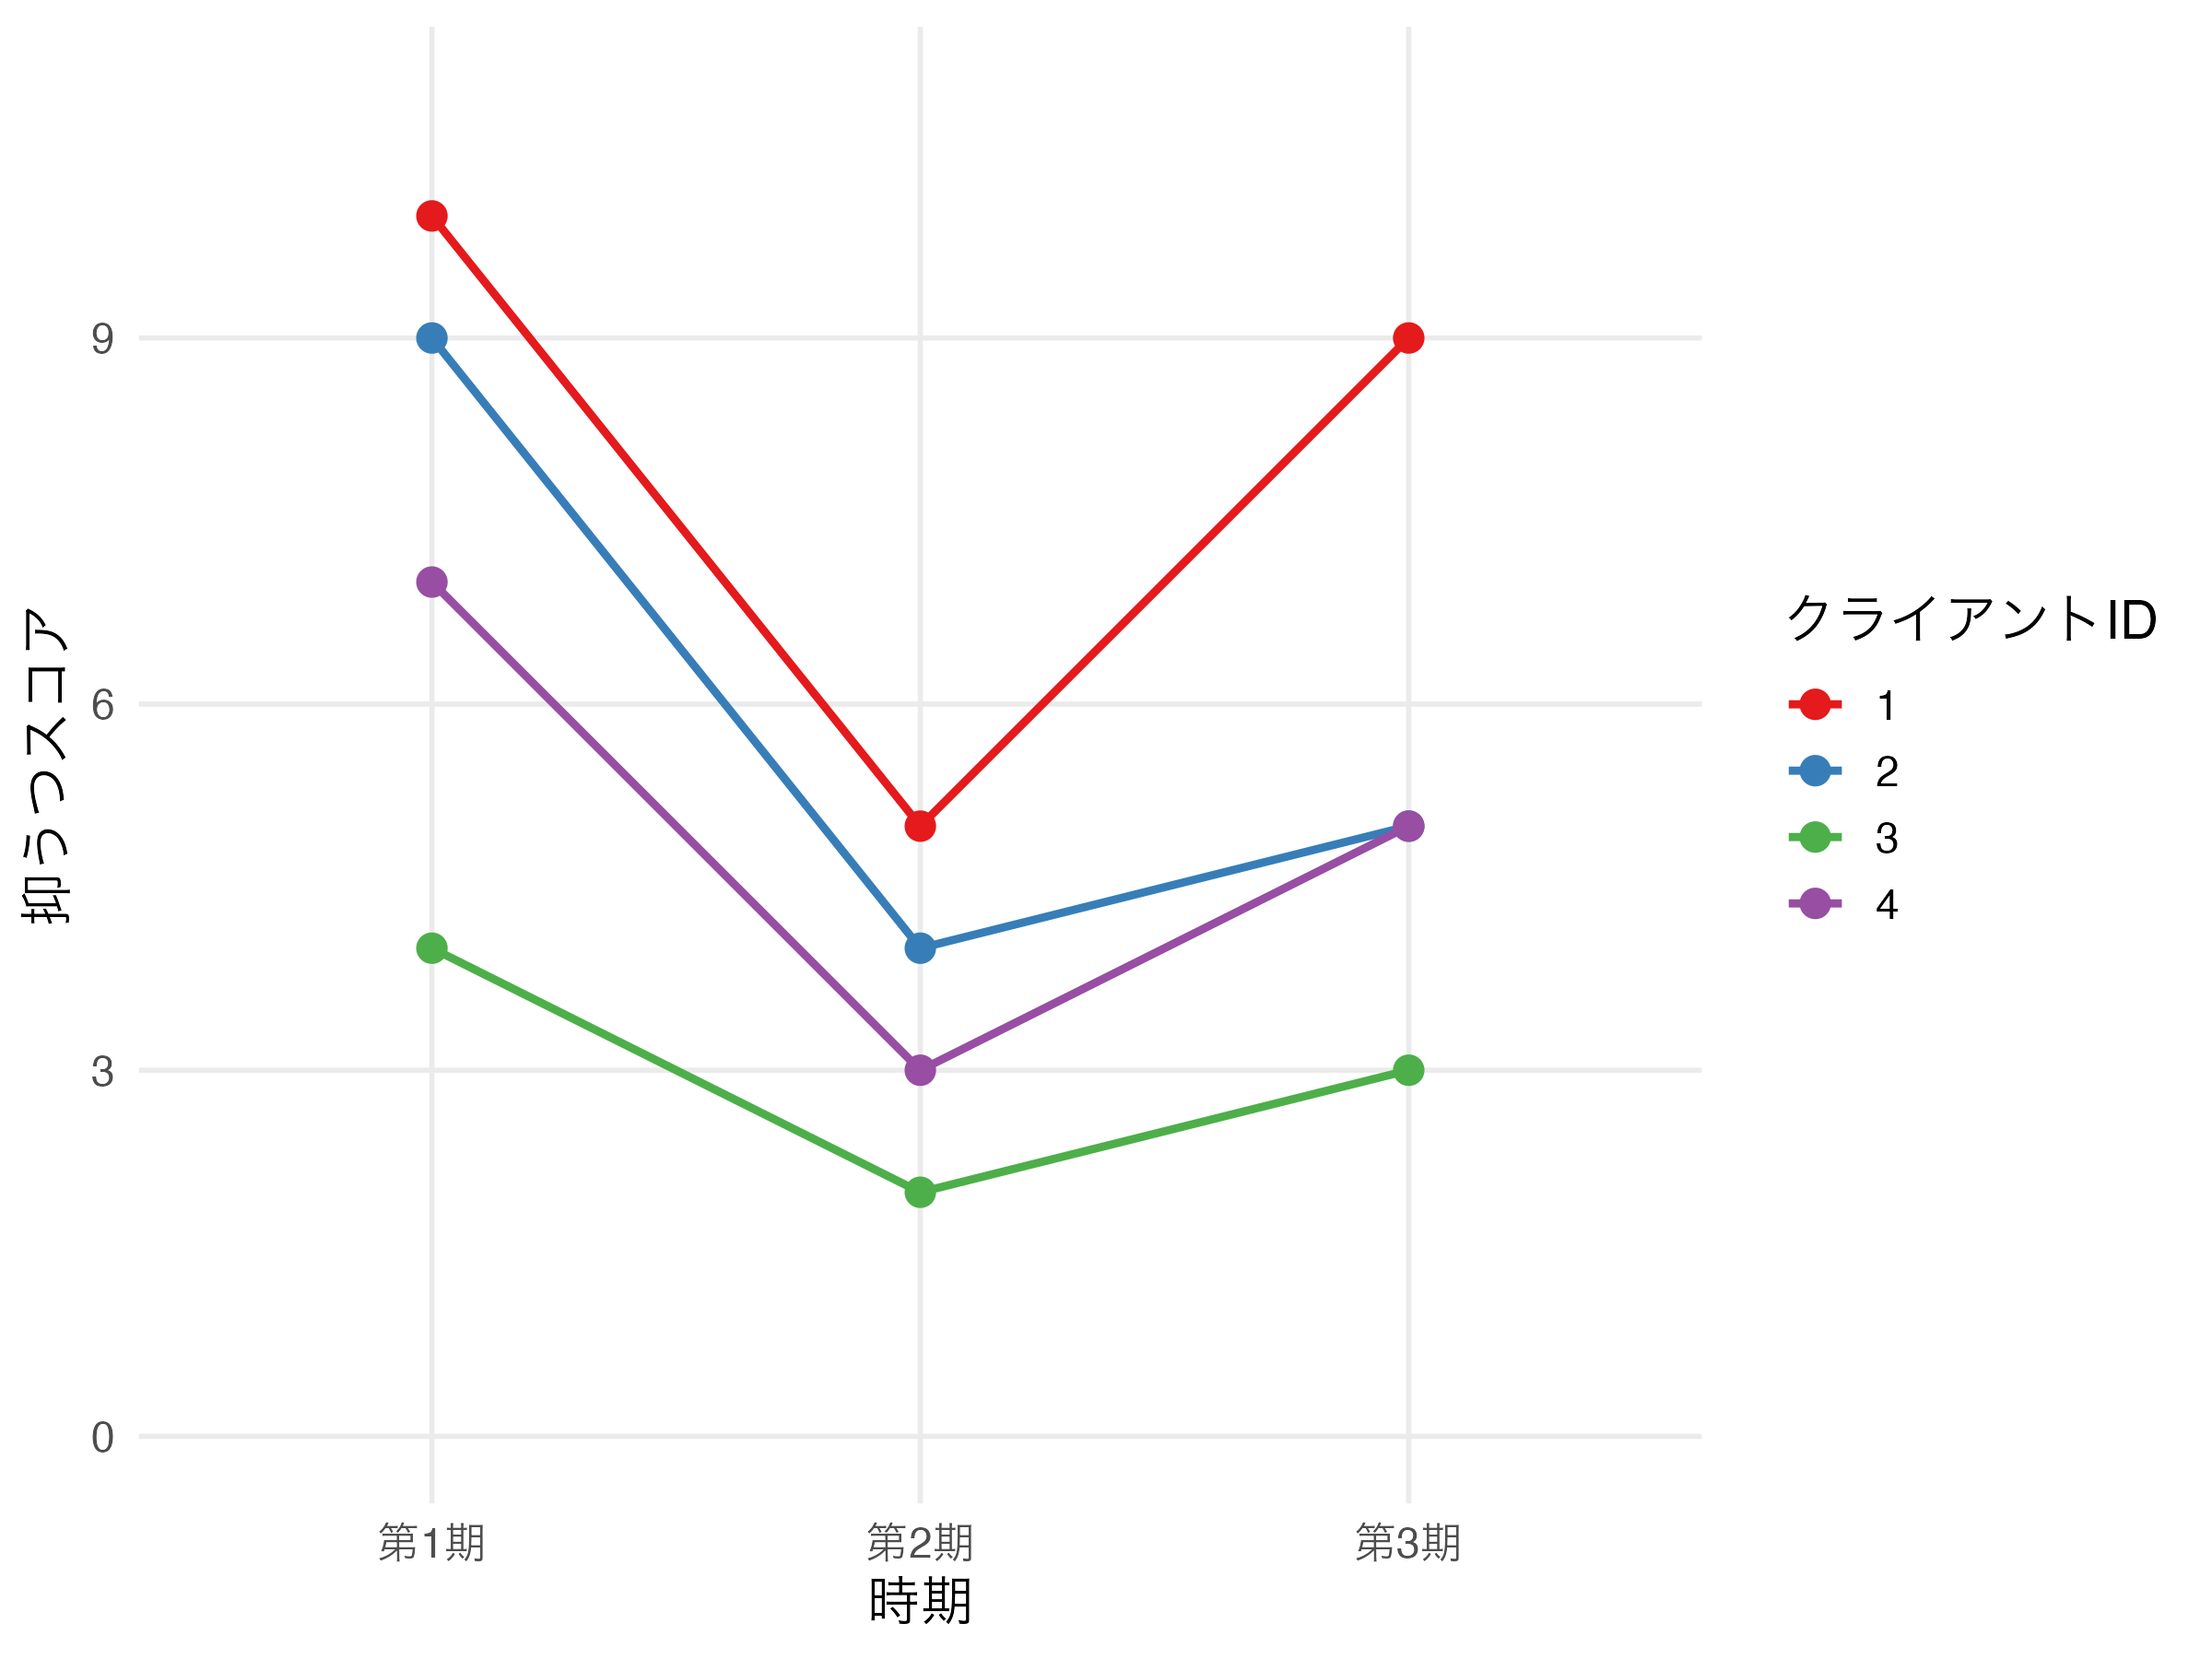
\includegraphics[keepaspectratio,width=\linewidth]{figures/21_Within/Within_pattern.png}
		\caption{介入効果によるクライアントの状態変化}
		\label{fig:21_01}
	\end{minipage}
	\hfill
	\begin{minipage}[t]{0.48\linewidth}
		\centering
		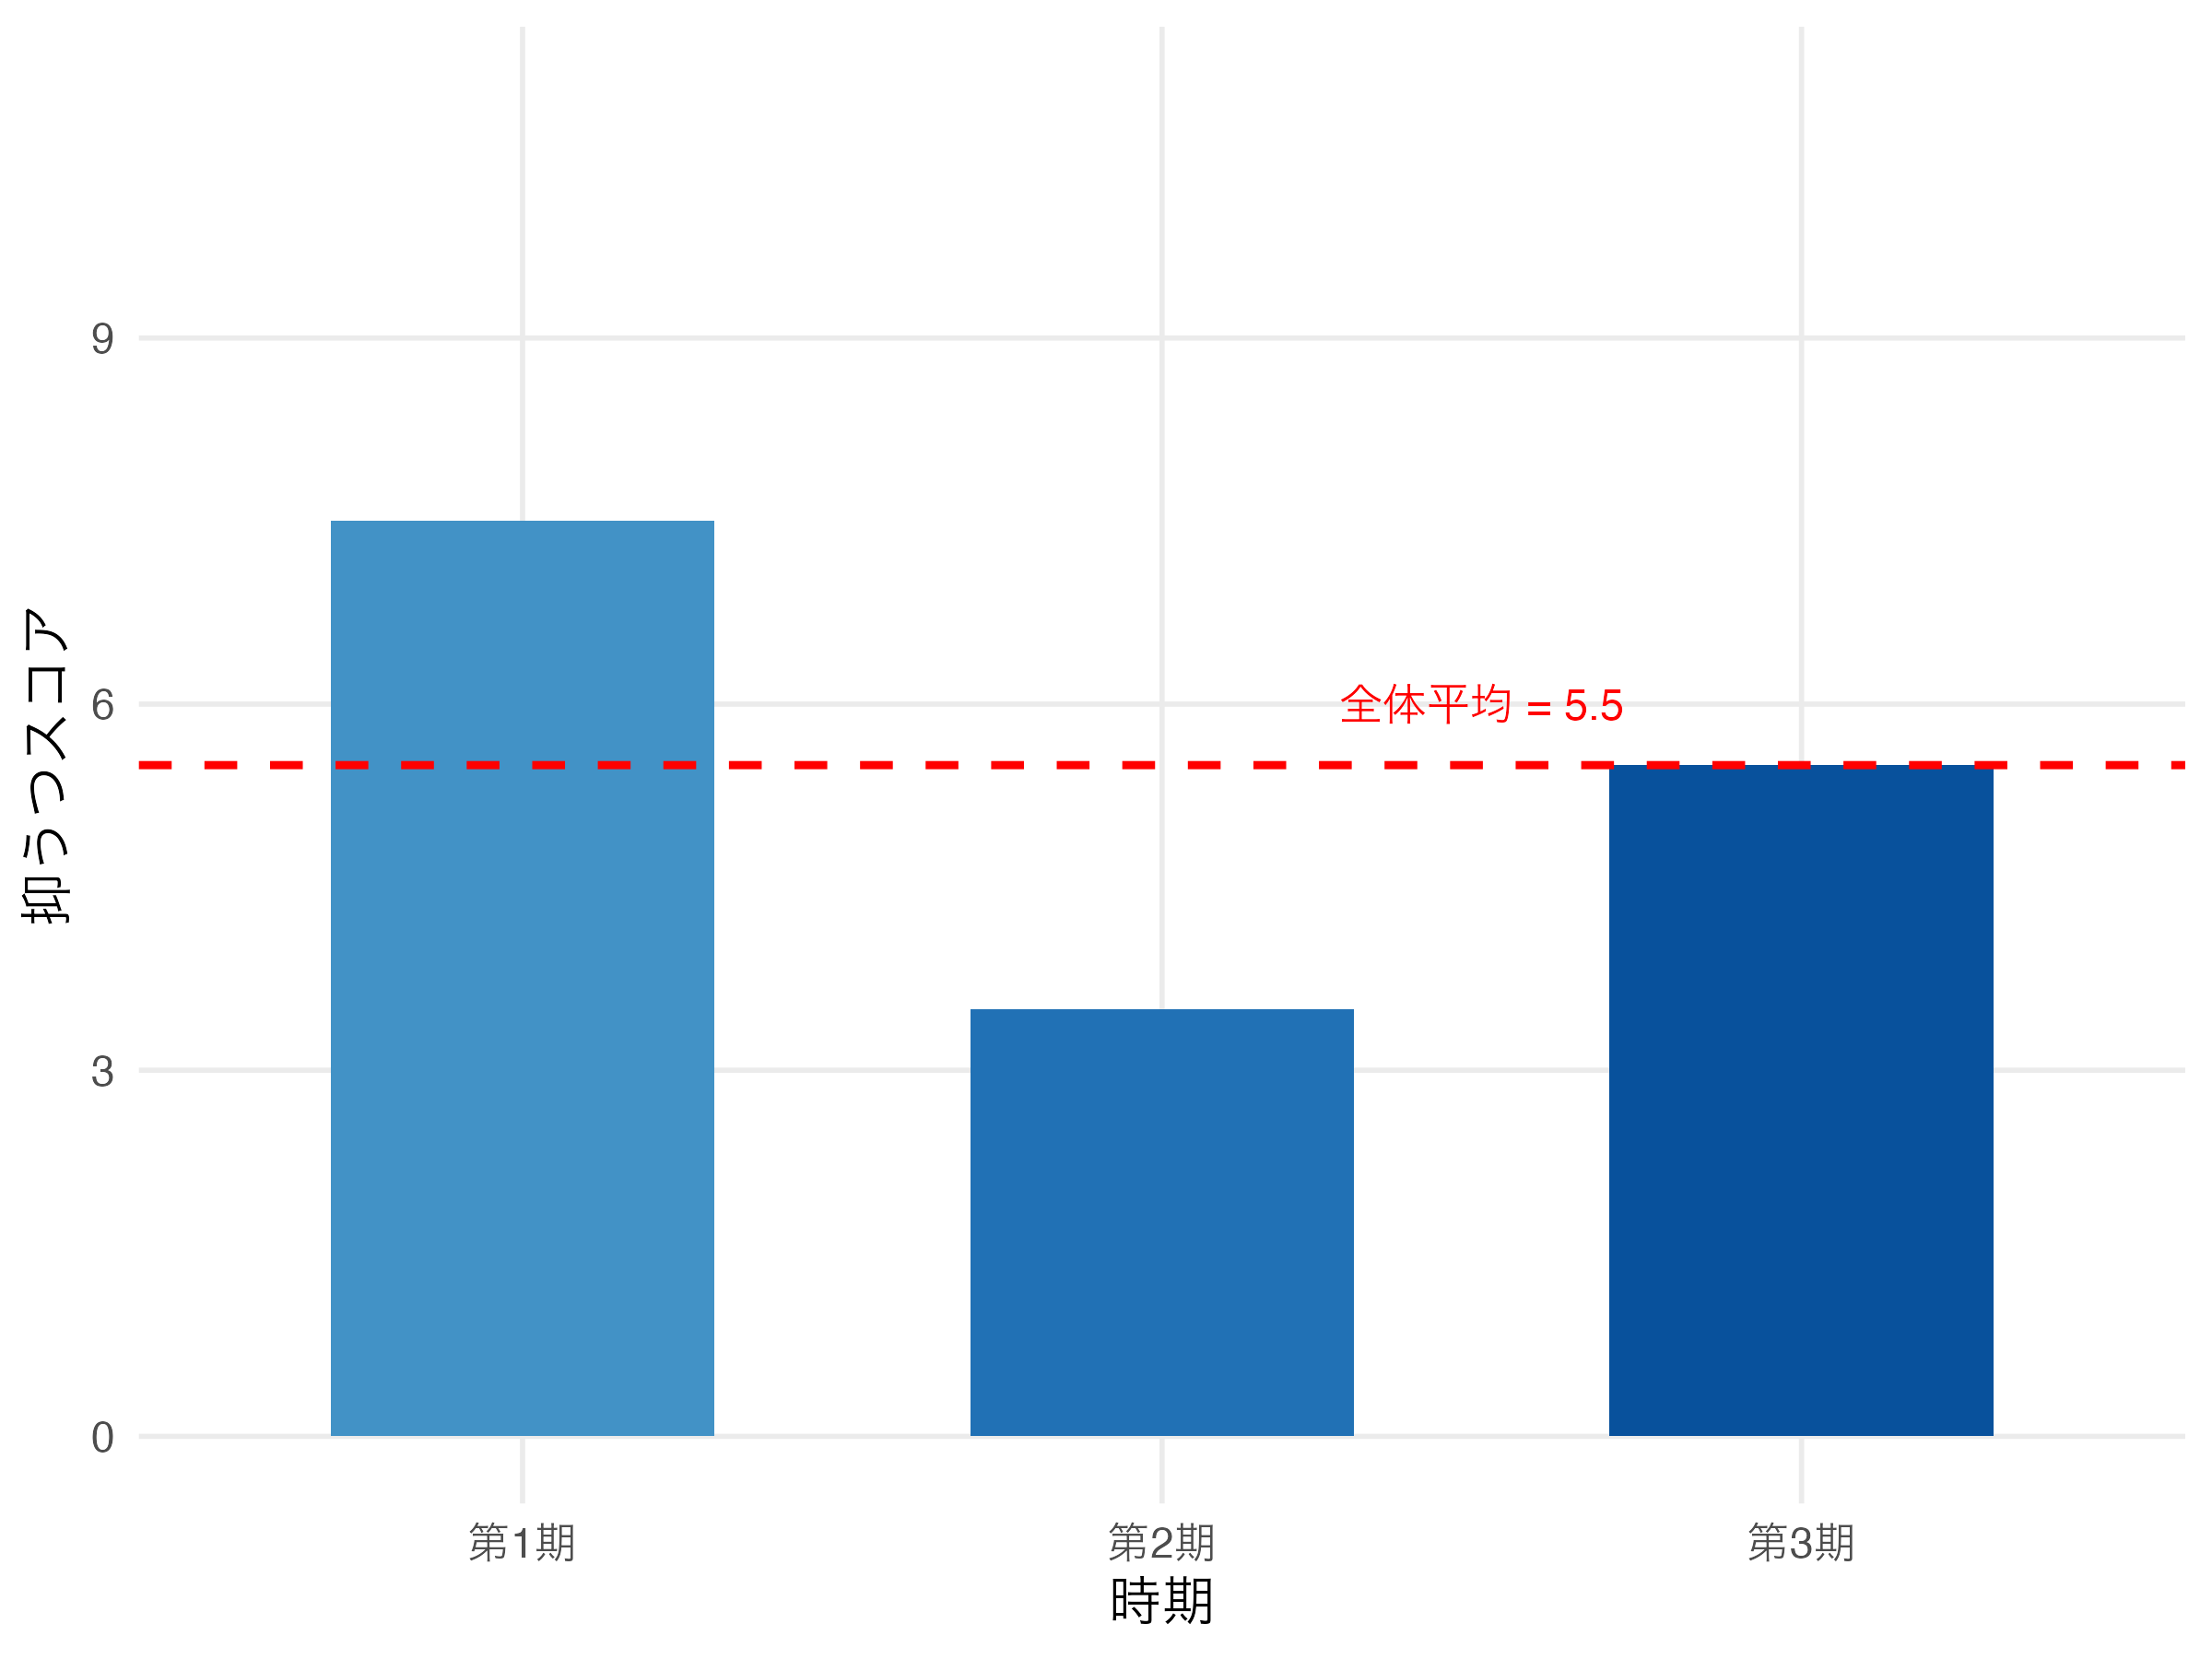
\includegraphics[keepaspectratio,width=\linewidth]{figures/21_Within/Within_mean.png}
		\caption{介入効果の可視化；全体平均と水準の比較}
		\label{fig:21_02}
	\end{minipage}
\end{figure}


% latex table generated in R 4.0.2 by xtable 1.8-4 package
% Fri Sep 11 14:57:29 2020
\begin{table}[h]
	\centering
	\caption{水準ごとの平均から効果を考える}
	\begin{tabular}{lrrr|r}
		\hline
		ID & Time1 & Time2 & Time3 & 平均  \\
		\hline
		1  & 10    & 5     & 9     & 8   \\
		2  & 9     & 4     & 5     & 6   \\
		3  & 4     & 2     & 3     & 3   \\
		4  & 7     & 3     & 5     & 5   \\
		\hline
		平均 & 7.5   & 3.5   & 5.5   & 5.5 \\\hline
	\end{tabular}
	\label{tbl::21_02}
\end{table}

図\ref{fig:21_02}は，水準ごとの平均値と全体平均を比較したものです。各水準の平均値が全体平均からどれだけ離れているか，というのが効果の大きさになります。第一期(Time1)は全体平均より高く，第二期(Time2)は低く，第三期(Time3)はほぼ同じ，ということがわかりますね。

さて，次に考えたいのは，「個人差こそあれ」のところです。\keytermL{個人差}{こじんさ}とは，効果に関係なく，各人がもともと持っている特性や状態の違いを指します。たとえば，表\ref{tbl::21_01}のデータを見ると，ID=1の人は全体的にスコアが高く，ID=3の人は全体的にスコアが低い，という傾向が見られます。個人の平均を図にしてみるとその違いは明らかです(図\ref{fig:21_03})。
今回この差分は個人によるものであって，見たい介入効果の部分ではありません。見たい効果は「時期」要因による，3つの水準それぞれへの影響，$\beta_j$ です。数式的に表現すると，個人$i$ の第$j$期におけるデータ$y_{ij}$は，次のように表すことができます。

\[ y_{ij} = \beta_0 + \delta_i + \beta_j X_{ij} + \epsilon_{ij} \]

ここで$X_{ij}$はまたしても，第$j$期に$\beta_j$の効果がある($1$)かない($0$)かを表している記号だと思ってください。また，ポイントとして，新たに$\delta_i$というのが出てきていることに注意してください。これは$i$に伴って変わる数字で，時期$j$の添字がついていませんから，「時期を通して一貫した個人の平均値」ということになります。$\beta_0$は$i$も$j$もついていませんから，個人にも時期にも関係なく変化しない全体の平均値を表しています。

具体的な数字で見てみましょう。ID=1の人について考えると，この人のデータは第1期では$10$，第2期では$5$，第3期では$9$でした。全体平均が$5.5$ですから，この人の個人差$\delta_1$は$+2.5$になります。時期の効果$\beta_j$は，第1期では$+2.0$，第2期では$-2.0$，第3期では$0.0$ですから，第1期のデータは次のように表せます。

\[ 10 = 5.5 + 2.5 + 2.0 + \epsilon_{11} \]

ここで$\epsilon_{11}$は誤差項で，逆算すると$0.0$であることがわかります。この人のこの時期のポイントは，誤差なく理論通りの値が出たことになります。

同様に，第2期，第3期も表してみましょう。

\[ 5 = 5.5 + 2.5 - 2.0 + \epsilon_{12} \]
\[ 9 = 5.5 + 2.5 + 0.0 + \epsilon_{13} \]

ここで，$\epsilon_{12}$は$-1.0$，$\epsilon_{13}$は$+1.0$です。理論と実測のズレはこの介入ではわからない要素なので，これを誤差と考えるほかありません。この計算を図で表したのが図\ref{fig:21_04}です。

\begin{figure}[h]
	\centering
	\begin{minipage}[t]{0.48\linewidth}
		\centering
		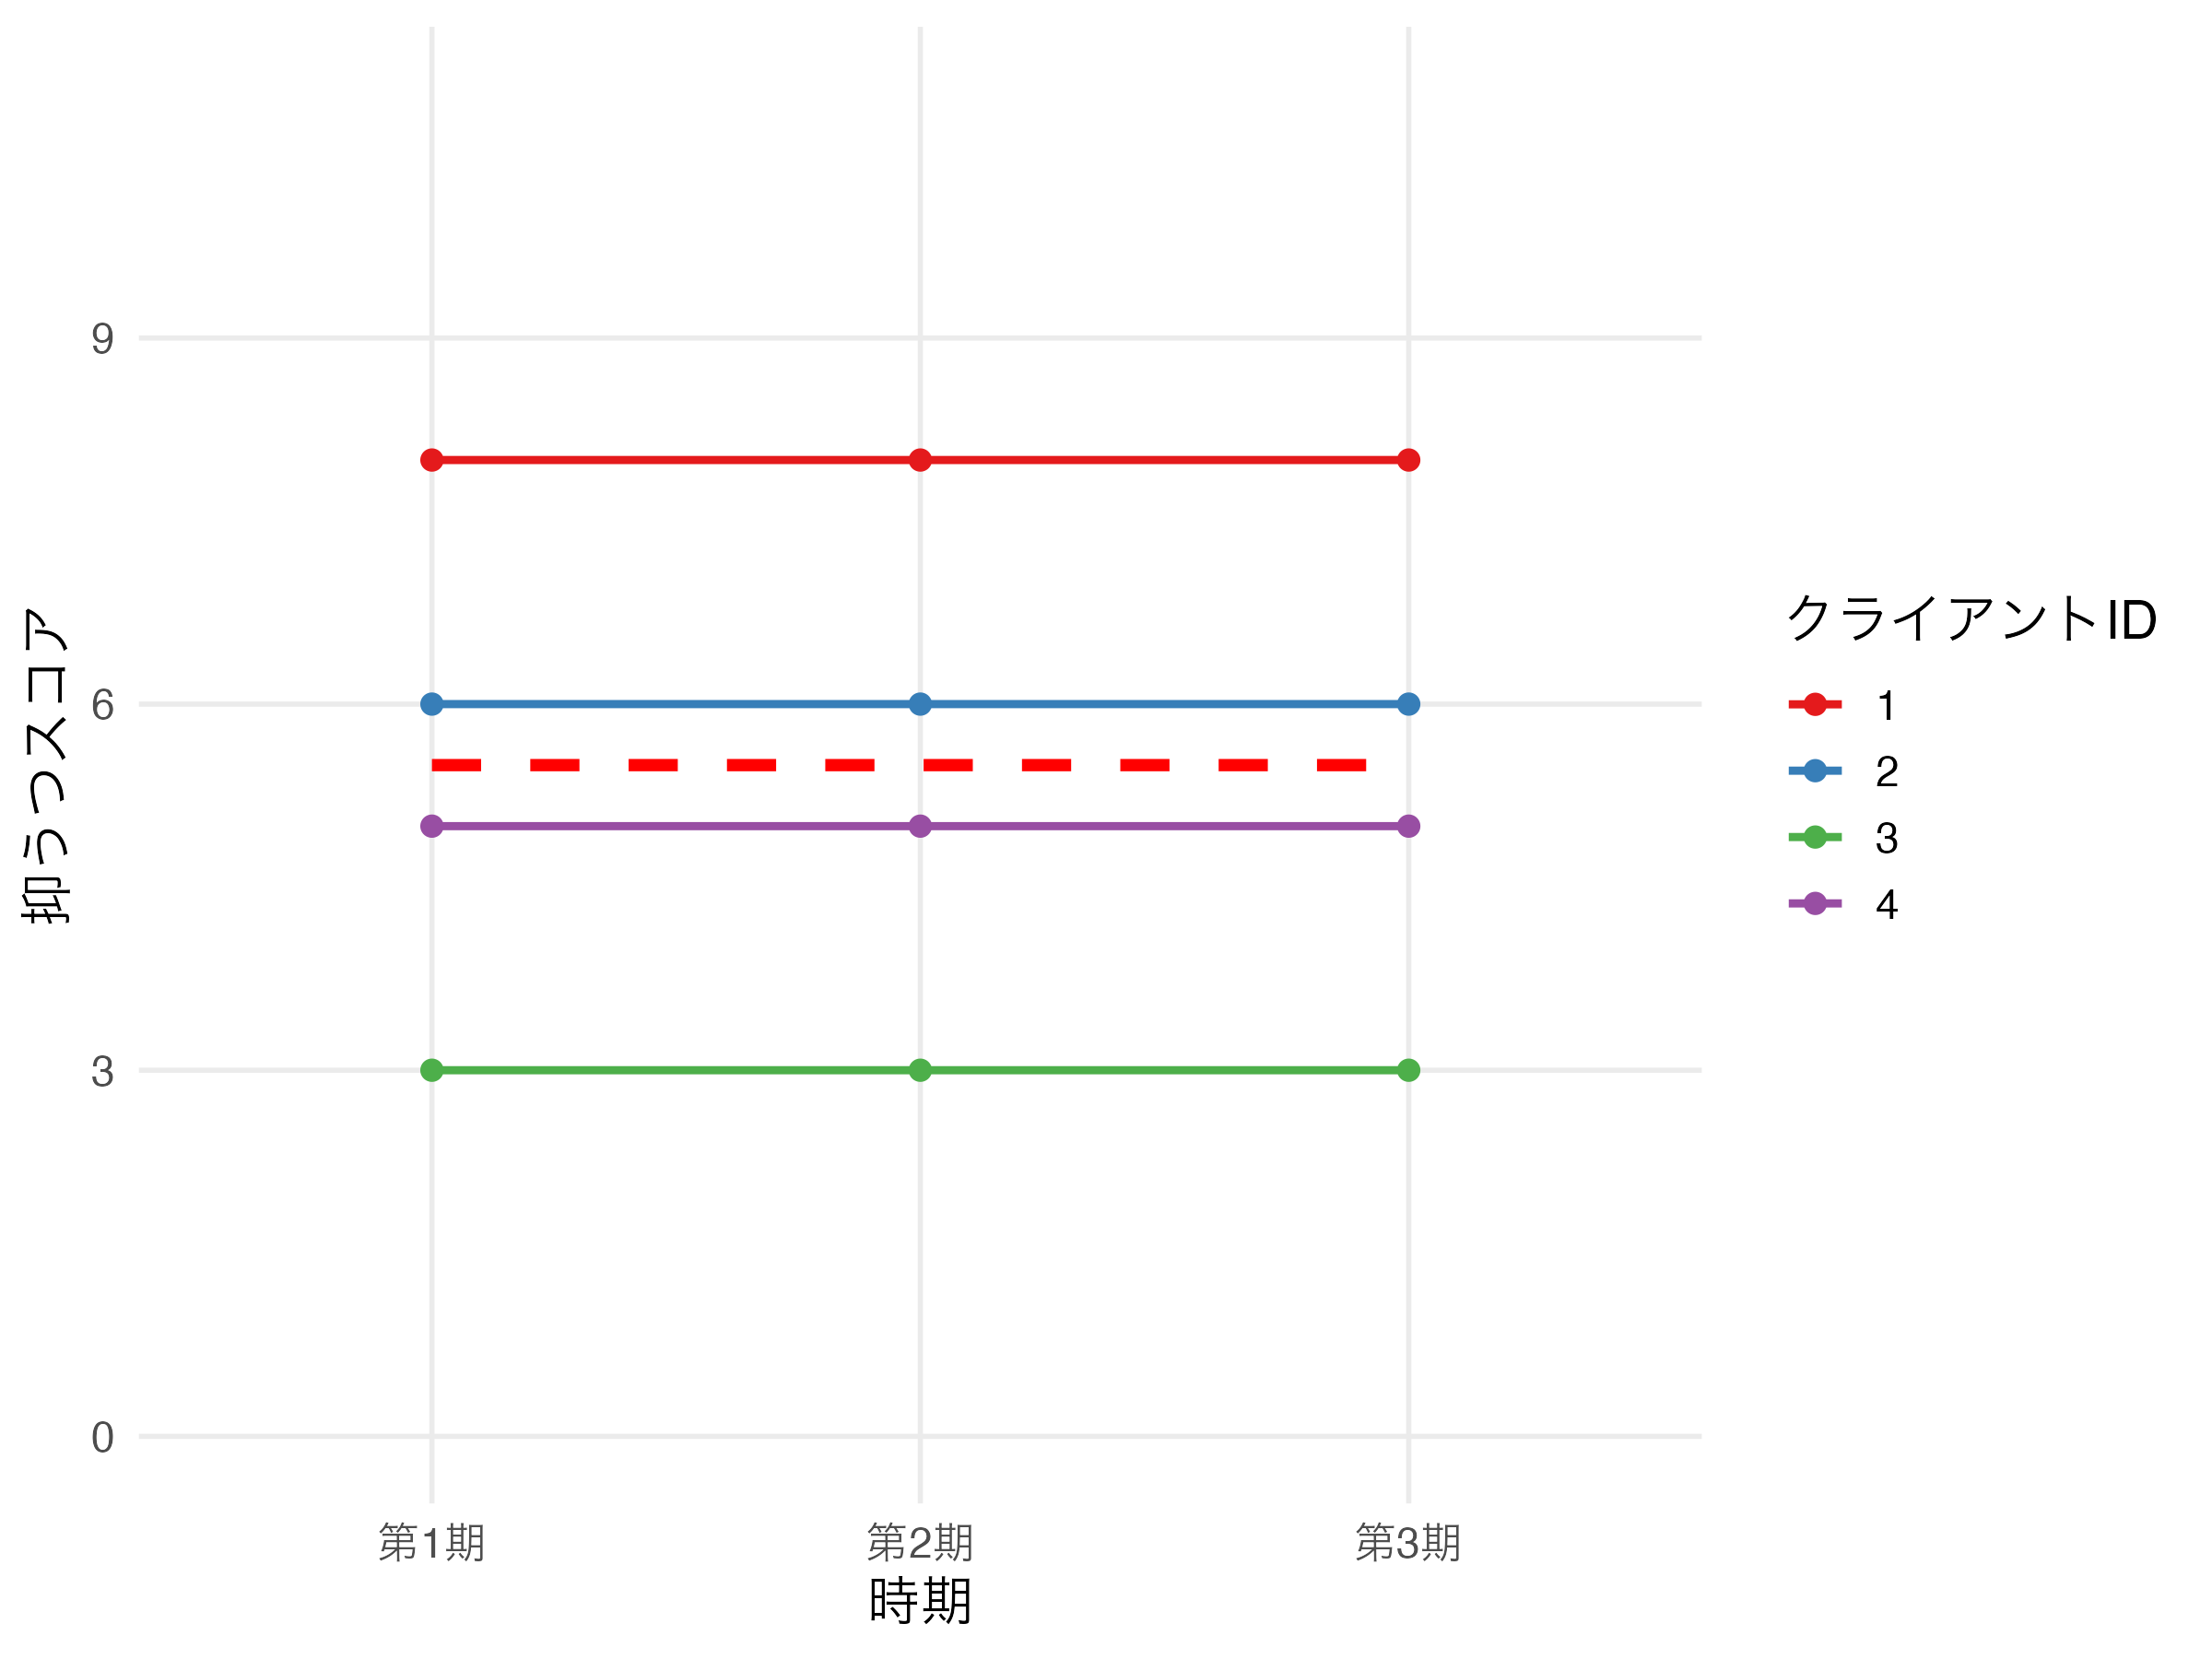
\includegraphics[keepaspectratio,width=\linewidth]{figures/21_Within/Within_individual.png}
		\caption{個人が持っている特性の違い(個人差)の考慮}
		\label{fig:21_03}
	\end{minipage}
	\hfill
	\begin{minipage}[t]{0.48\linewidth}
		\centering
		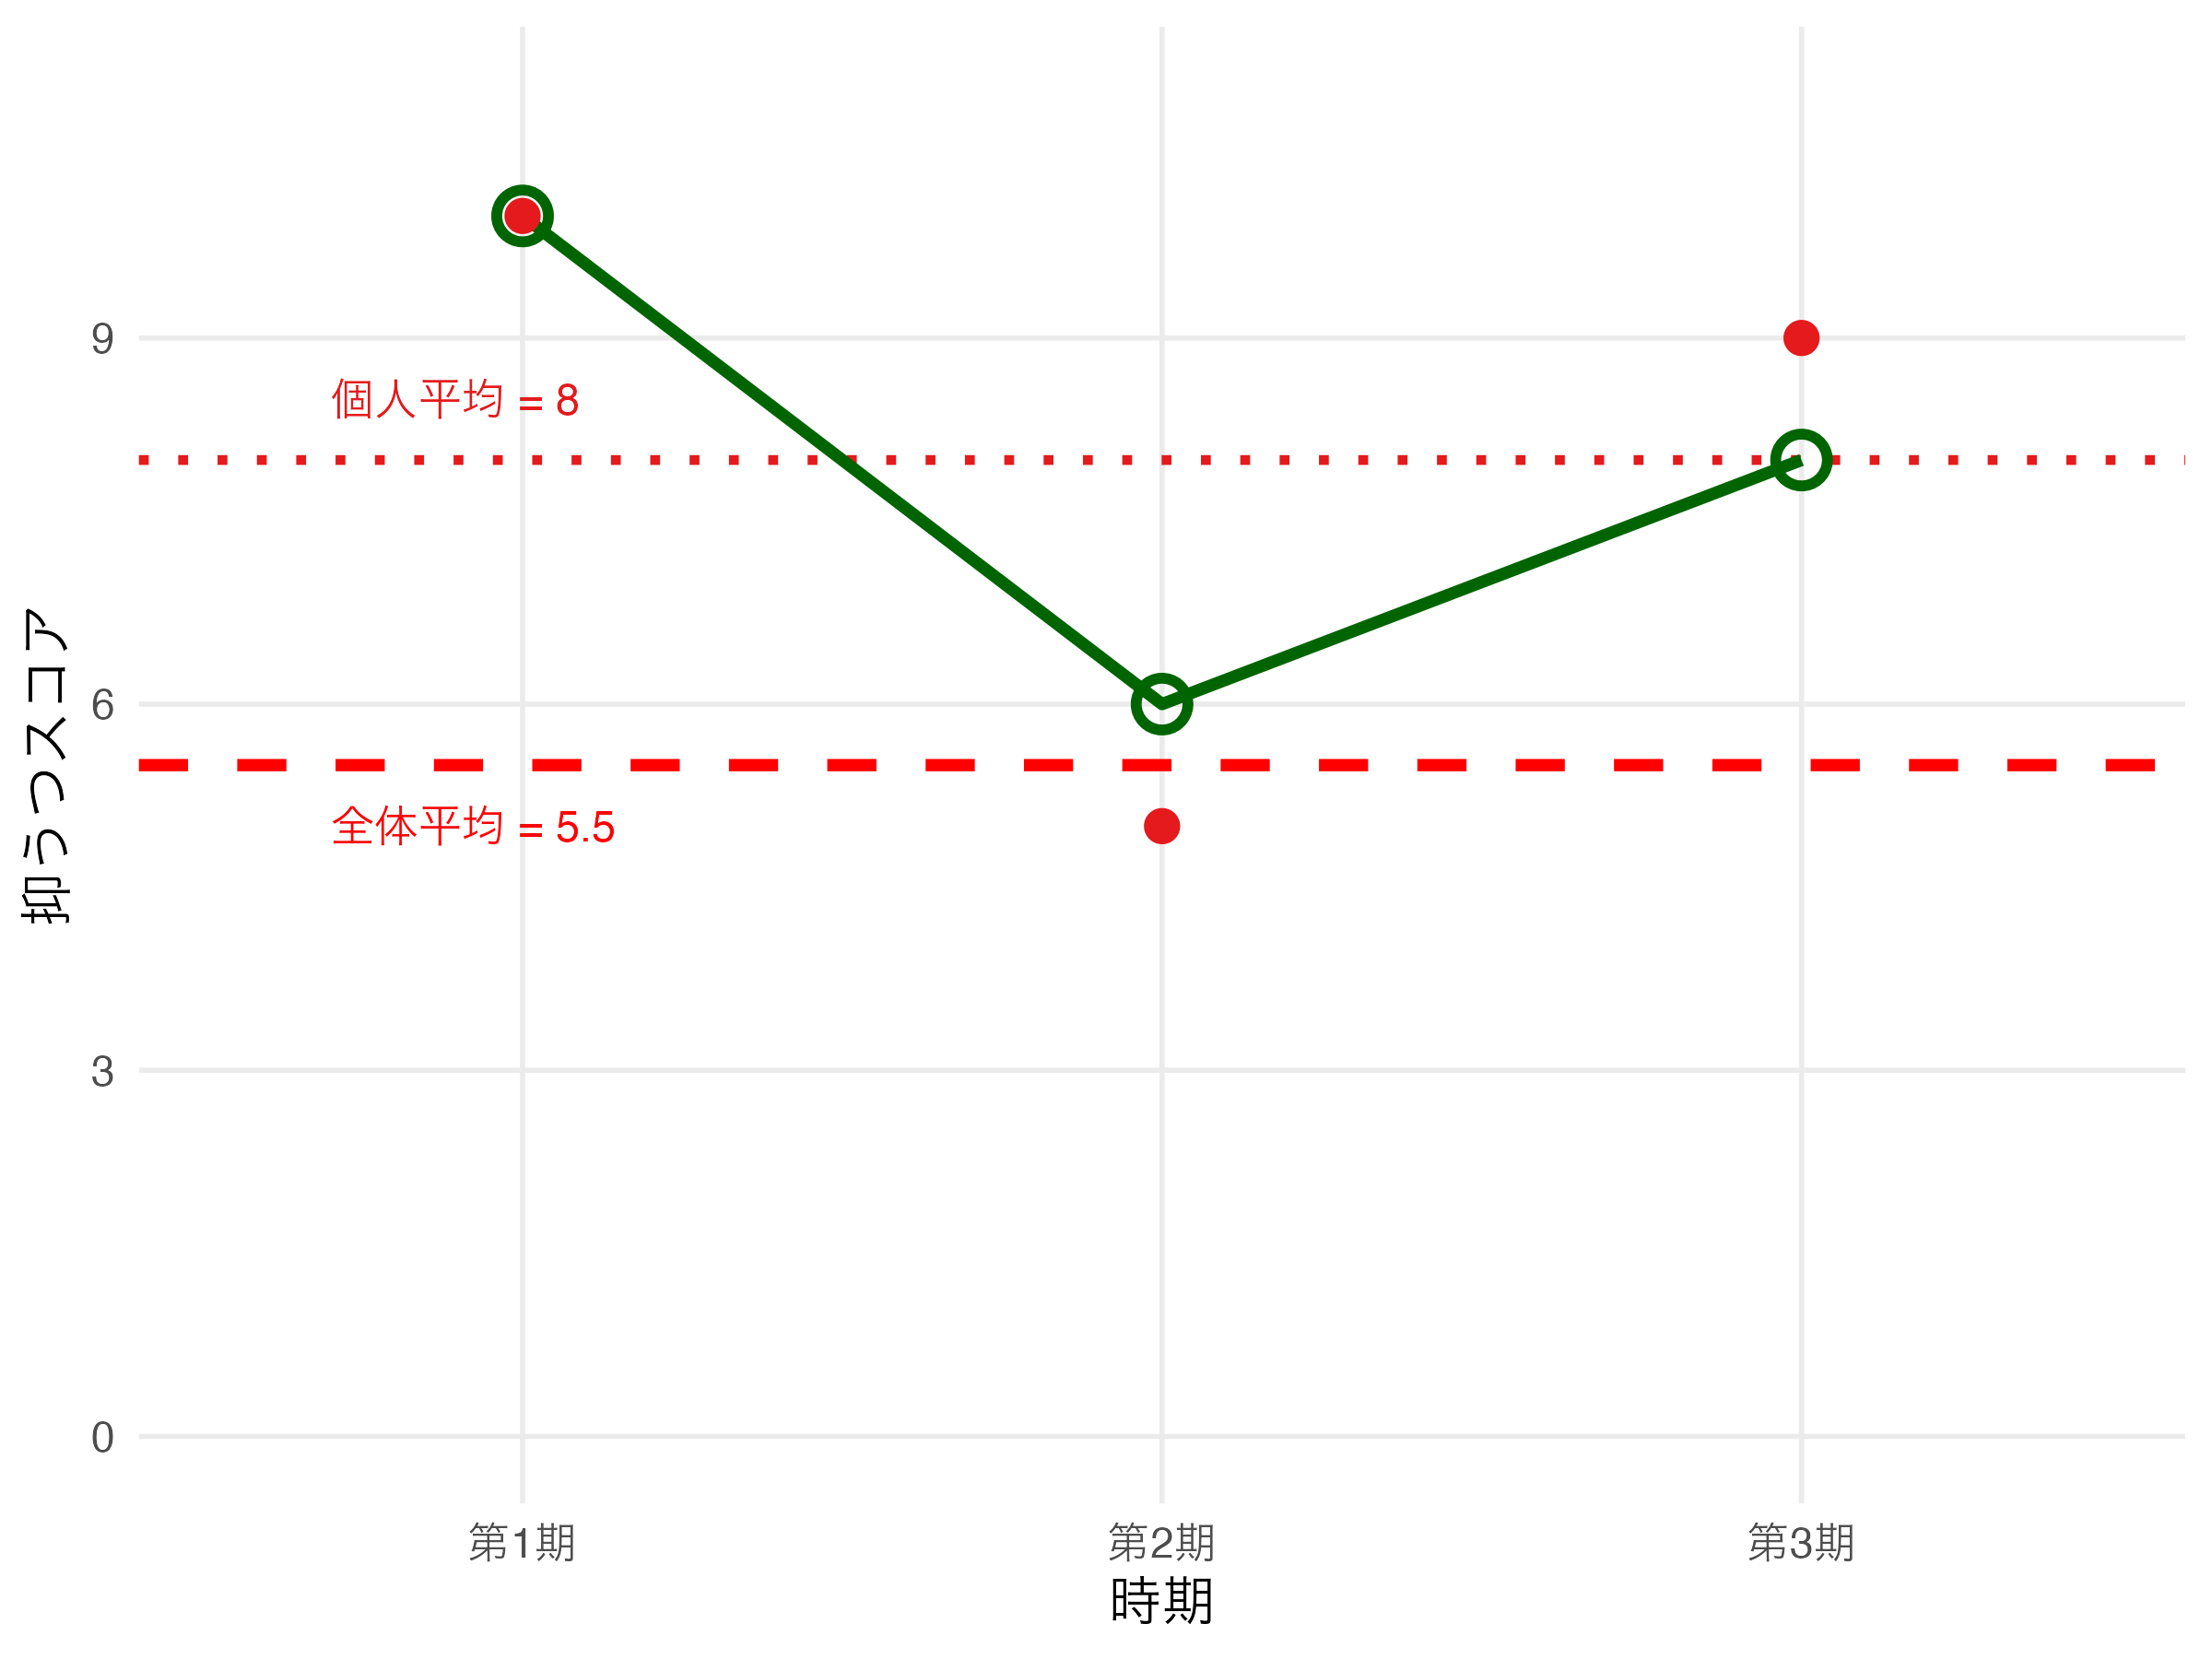
\includegraphics[keepaspectratio,width=\linewidth]{figures/21_Within/Within_model_id1.png}
		\caption{ID=1のデータのモデル化}
		\label{fig:21_04}
	\end{minipage}
\end{figure}


この計算を全員に対して行い，効果，個人差，誤差を計算して表にしたのが表\ref{tbl::21_03}です。例によって総和すると0ですので，平方和を計算することで相対的な大きさを比較できるようになります。

% latex table generated in R 4.0.2 by xtable 1.8-4 package
% Fri Sep 11 15:52:17 2020
\begin{table}[h]
	\centering
	\caption{効果，個人差，誤差を析出する}
	\begin{tabular}{llrcrrr}
		\hline
		ID  & 時期    & スコア & 全体平均 & 個人差  & 効果   & 誤差   \\
		\hline
		1   & Time1 & 10  & 5.5  & +2.5 & +2.0 & 0.0  \\
		1   & Time2 & 5   & 5.5  & +2.5 & -2.0 & -1.0 \\
		1   & Time3 & 9   & 5.5  & +2.5 & 0.0  & +1.0 \\
		2   & Time1 & 9   & 5.5  & +0.5 & +2.0 & +1.0 \\
		2   & Time2 & 4   & 5.5  & +0.5 & -2.0 & 0.0  \\
		2   & Time3 & 5   & 5.5  & +0.5 & 0.0  & -1.0 \\
		3   & Time1 & 4   & 5.5  & -2.5 & +2.0 & -1.0 \\
		3   & Time2 & 2   & 5.5  & -2.5 & -2.0 & +1.0 \\
		3   & Time3 & 3   & 5.5  & -2.5 & 0.0  & 0.0  \\
		4   & Time1 & 7   & 5.5  & -0.5 & +2.0 & 0.0  \\
		4   & Time2 & 3   & 5.5  & -0.5 & -2.0 & 0.0  \\
		4   & Time3 & 5   & 5.5  & -0.5 & 0.0  & 0.0  \\
		\hline\hline
		平方和 &       &     &      & 39.0 & 32.0 & 6.0  \\\hline
	\end{tabular}
	\label{tbl::21_03}
\end{table}

ここにあるように，個人$i$の時期$j$における誤差，と各セルに細かく誤差が計算できるようになりました。これが群内要因計画の強みなのです。

\section{群内モデルの平方和の分解}

それではこの数値を元に，平方和の分解を確認してみましょう。群内要因計画の場合，総平方和$SS_T$は，効果による平方和$SS_A$，個人差による平方和$SS_S$，および誤差による平方和$SS_E$に分解されます。
\[ SS_T = SS_A + SS_S + SS_E \]

上の数値例でいうと，次のような等式が成り立っていることがわかります。

\[ 77.0 = 32.0 + 39.0 + 6.0 \]

これが群内要因の平方和の分解です。これを元に「意思決定」，つまり効果があるかどうかの判断をするわけですが，そのためには平方和(SS)から平均平方(MS)を計算しなければなりません。群間要因の時にやったように，平均平方にするには一水準あたりの平方和を考えることになりますから，それぞれの要因がどれだけの自由度を持っているかを考えなければなりません。
効果$SS_A$は3水準ですから，自由度は$3-1=2$です。個人差$SS_S$は4人ですから，自由度は$4-1=3$です。誤差$SS_E$は全体の自由度$12-1=11$から，効果と個人差の自由度を引いたものですから，$11-2-3=6$となります。
これを元に平均平方を計算すると，次のようになります。
\begin{itemize}
    \item 効果の平均平方：$MS_A = SS_A / df_A = 32.0 / 2 = 16.0$
    \item 個人差の平均平方：$MS_S = SS_S / df_S = 39.0 / 3 = 13.0$
    \item 誤差の平均平方：$MS_E = SS_E / df_E = 6.0 / 6 = 1.000$
\end{itemize}
これを元にF値を計算します。群内要因計画の場合，効果のF値は，効果の平均平方を誤差の平均平方で割ったものになります。
\[ F = \frac{MS_A}{MS_E} = \frac{16.0}{1} =16.00 \]
このF値を元に，効果が有意かどうかを判断します。分散の比の分布であるF分布で，今回は分子の自由度が$2$，分母の自由度が$6$ですから，理論値は$5.143253$になります\footnote{Rで\verb|qf(0.95,2,6)|とすれば計算できます。}。今回の16はこれに比べてかなり大きいので，有意である(3つの水準間の平均値は同じではない)，と判断できます。

最後に分散分析表にこのことをまとめておきましょう。表\ref{tbl::21_04}がその分散分析表です。
\begin{table}[h]
    \centering
    \caption{群内要因計画の分散分析表}
    \begin{tabular}{lrrrrr}
        \hline
        要因      & 平方和(SS) & 自由度(df) & 平均平方(MS) & F値    & p値  \\
        \hline
        個人差    & 39.0       & 3          & 13.0        &        &      \\
        \hline
        効果      & 32.0       & 2          & 16.0        & 16.00  &  0.0039\\
        誤差      & 6.0        & 6          & 1.000       &        &      \\
        \hline
        総和      & 77.0       & 11         &             &        &      \\
        \hline
    \end{tabular}
    \label{tbl::21_04}
\end{table}

\section{群間計画と群内計画の比較}
ここで\keyterm{群間要因}{ぐんかんよういん}{between design}計画と\keyterm{群内要因}{ぐんないよういん}{within design}計画の構造的な違いに触れておきたいと思います。

群内計画では，個人が誰であるかという情報があったので個人差を算出でき，それに基づいて分析しました。
が，群内計画の時のデータを群間計画のように分析してみるとどうなるでしょうか。表\ref{tbl::21_03}にある数字が同じであれば，群内計画であれ群間計画であれ，当然全体の平方和(分散)は同じです。ただ個人情報が抜けているのであれば，効果と誤差にしか分割できません。言い換えると，群間計画というのは誤差の中に個人差が含まれており，「これは誤差なのかな，個人差なのかな？ 」という区別がつかない状態である，ということです(図\ref{fig:21_05})。

群間・群内どちらの計画であっても，最終的には，誤差の大きさに対して効果の大きさはどうか，という観点から評価します\footnote{統計的な評価，価値判断の方法については後期の推測統計学で扱うので，ここでは比較して考える要素が何であるかを理解していただければ十分です。}。効果の大きさ＝分子が同じデータであれば，分母が小さい方が相対的に大きいと判断されることになりますね。群間計画の時の誤差は偶然誤差と個人差を含んでおり，群内計画の時は個人差を含みませんから，\underline{群内計画の方が群間計画よりも，分析の精度が高い}ということになります。これは間違いなくそうなのです。

であれば，すべての研究が群内計画であればよいのに，と思うかもしれません。ただし現実的な問題として，同じ人に何度も何度もデータを提供してもらうのは，非常に負担をかけることになります(群内計画は反復測定計画とも呼ばれるのでした)。研究倫理的な観点，あるいは計画上の手間を考えると，群間計画にせざるを得ないということが少なくありません。研究者，研究に協力してくれる人，のコストを考えて実験計画はデザインする必要があるということです。

\begin{figure}[h]
	\centering
	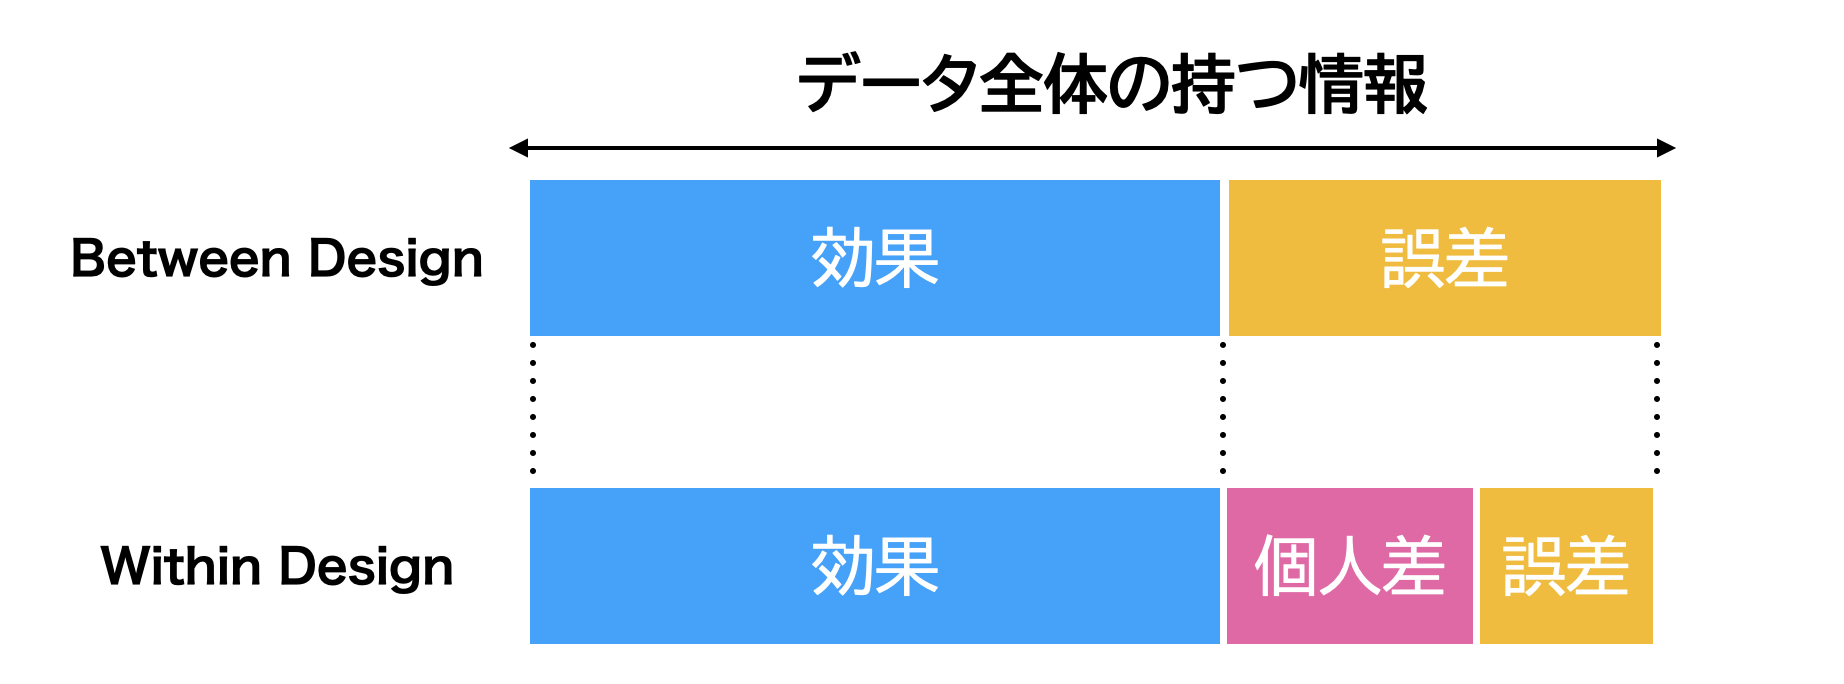
\includegraphics[keepaspectratio,width=0.8\linewidth]{figures/21_Within/Within_divide.png}
	\caption{群内計画と群間計画の違い}
	\label{fig:21_05}
\end{figure}


\section{発展的な話：確率分布としての線形モデル}
\label{thinkWithDistribution}
さて，ここで少し発展的な要素も含んだお話をしておきましょう。

要因計画がどのようなものであれ，データの散らばりを生んでいるのは効果，個人差，偶然誤差によるものだと考えるのでした。逆に言えば，これらがなければすべての値は同じになるはずだ，という観点から逆算し，効果，個人差，偶然誤差の大きさを見積もっていったのでした。

ここで，誤差を考える時には確率の考え方を利用してそれをコントロールする，という話を思い出してください。ガウスが考えた誤差論は，平均が$0$，分散$\sigma^2$で散らばる正規分布に従うのでした。すなわち誤差を$\epsilon_{i}$とすると，次のように表現できます。
\[ \epsilon_{i} \sim Normal(0, \sigma) \]


群間計画の場合は，各項目の値$y_i$を切片$\beta_0$と効果$\beta_1$と誤差に分けます。
\[ y_i = \beta_0 + \beta_1 + \epsilon_i \]
\[\epsilon_i \sim Normal(0, \sigma) \]

イメージでいうなら次のような形です。
\begin{figure}[h]
	\centering
	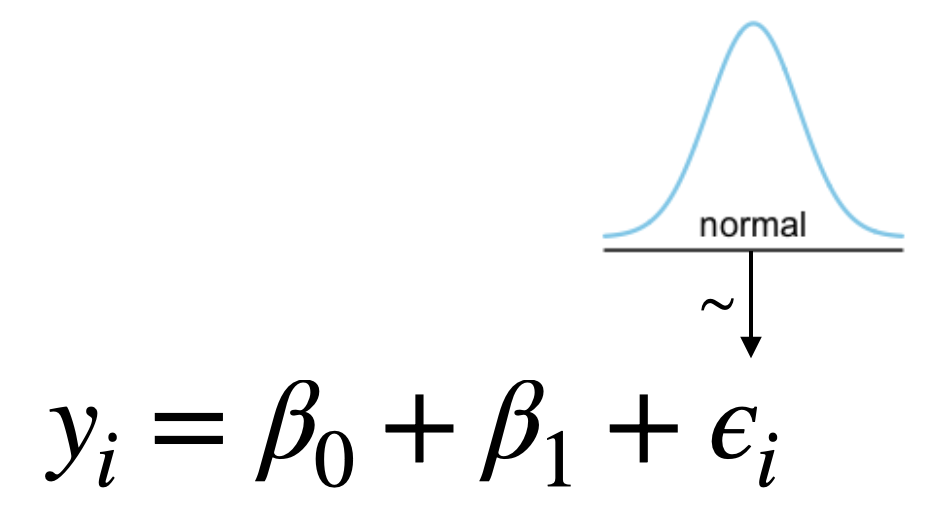
\includegraphics[keepaspectratio,width=0.45\linewidth]{figures/21_Within/between_eq.png}
\end{figure}

$\epsilon_i$が正規分布に従うのですが，$\beta_0+\beta_1$のところは確率的に変わるものではないことに注意してください。ここが確率的に変わらないということをよく考えれば，数式に沿ってある値が足されることと同じです。確率分布にある数字を加えると，その分布の位置がずれますね。正規分布は位置と幅でその特徴が作られているのですが，右辺全体で見ると，$\beta_0+\beta_1$のところは，正規分布の位置をずらすことでもあります。

ずれた分布は，正規分布の平均値が$\beta_0+\beta_1$ですから，式全体を整えると次のようになります。

\[ y_i \sim Normal(\beta_0+\beta_1 , \sigma) \]

この式のポイントは，$y=$ではなく$y\sim$になっているところです。データが正規分布に従う，という形に変わったのです。線形モデル(要因計画)はこのように，\textbf{確率分布の位置パラメータに数式(モデル)を当てはめる}こととも言えます。

さらにさらに。
群内計画の場合は，個人差$\delta_i$も計算できるのでした。この個人差というのも，たくさん集めると確率的な傾向を表してくるはずで，とくに個々人の生得的な性質に関係するのであれば，それはまた正規分布に従うと言えるでしょう。今回の個人差も相対的に捉えるので，平均をひとまず$\psi$とでも置いて\footnote{$\psi$はギリシア文字でプサイと読みます。大文字は$\Psi$であり，心理学Psychologyをギリシア語で表現した最初の文字になります。}，これを踏まえて表現すると次のようになります。
\[ \delta_i \sim Normal(\psi , \tau) \]

さてそうすると，群内計画の場合は2つの異なる正規分布が混ぜ合わさった形になっていることになります。式で書くと次のようになりますね。
\[ y_{ij} = \beta_0 + \delta_i + \beta_{ij} + \epsilon_{ij}\]
\[ \delta_i \sim N(\psi,\tau), \epsilon_{ij} \sim N(0,\sigma) \]

この式をイメージで表すと，次のような形になります。
\begin{figure}[h]
	\centering
	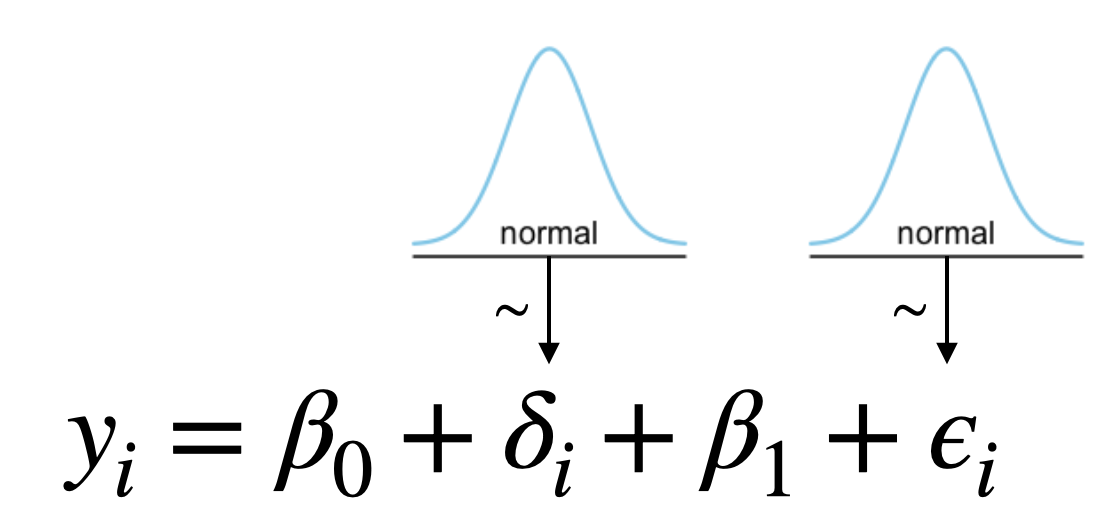
\includegraphics[keepaspectratio,width=0.45\linewidth]{figures/21_Within/within_eq.png}
\end{figure}

このように確率をふまえたモデルで考えると，群内計画のデータには2つの分布が混ざり込んでいることになりますから，\keyterm{混合効果モデル}{こんごうこうかもでる}{mixed effect model}と呼ぶことがあります。先ほどの群間計画では，$\beta_0+\beta_1$で平均値をずらした正規分布にデータが従うことになりましたが，群内計画では$\beta_0+\beta_1+\delta_i$がすでに確率的に分布し，それが平均値となった確率分布がデータの従う分布になる，つまり(誤差の)正規分布の中に(個人差の)正規分布が入れ子になった形でモデルが表現されたことになります。分布が混ざったので\textbf{混合}というのですね。先ほどのデータを使って図で表現するなら，図\ref{fig:21_06}のようになります。
\begin{figure}[h]
    \centering
    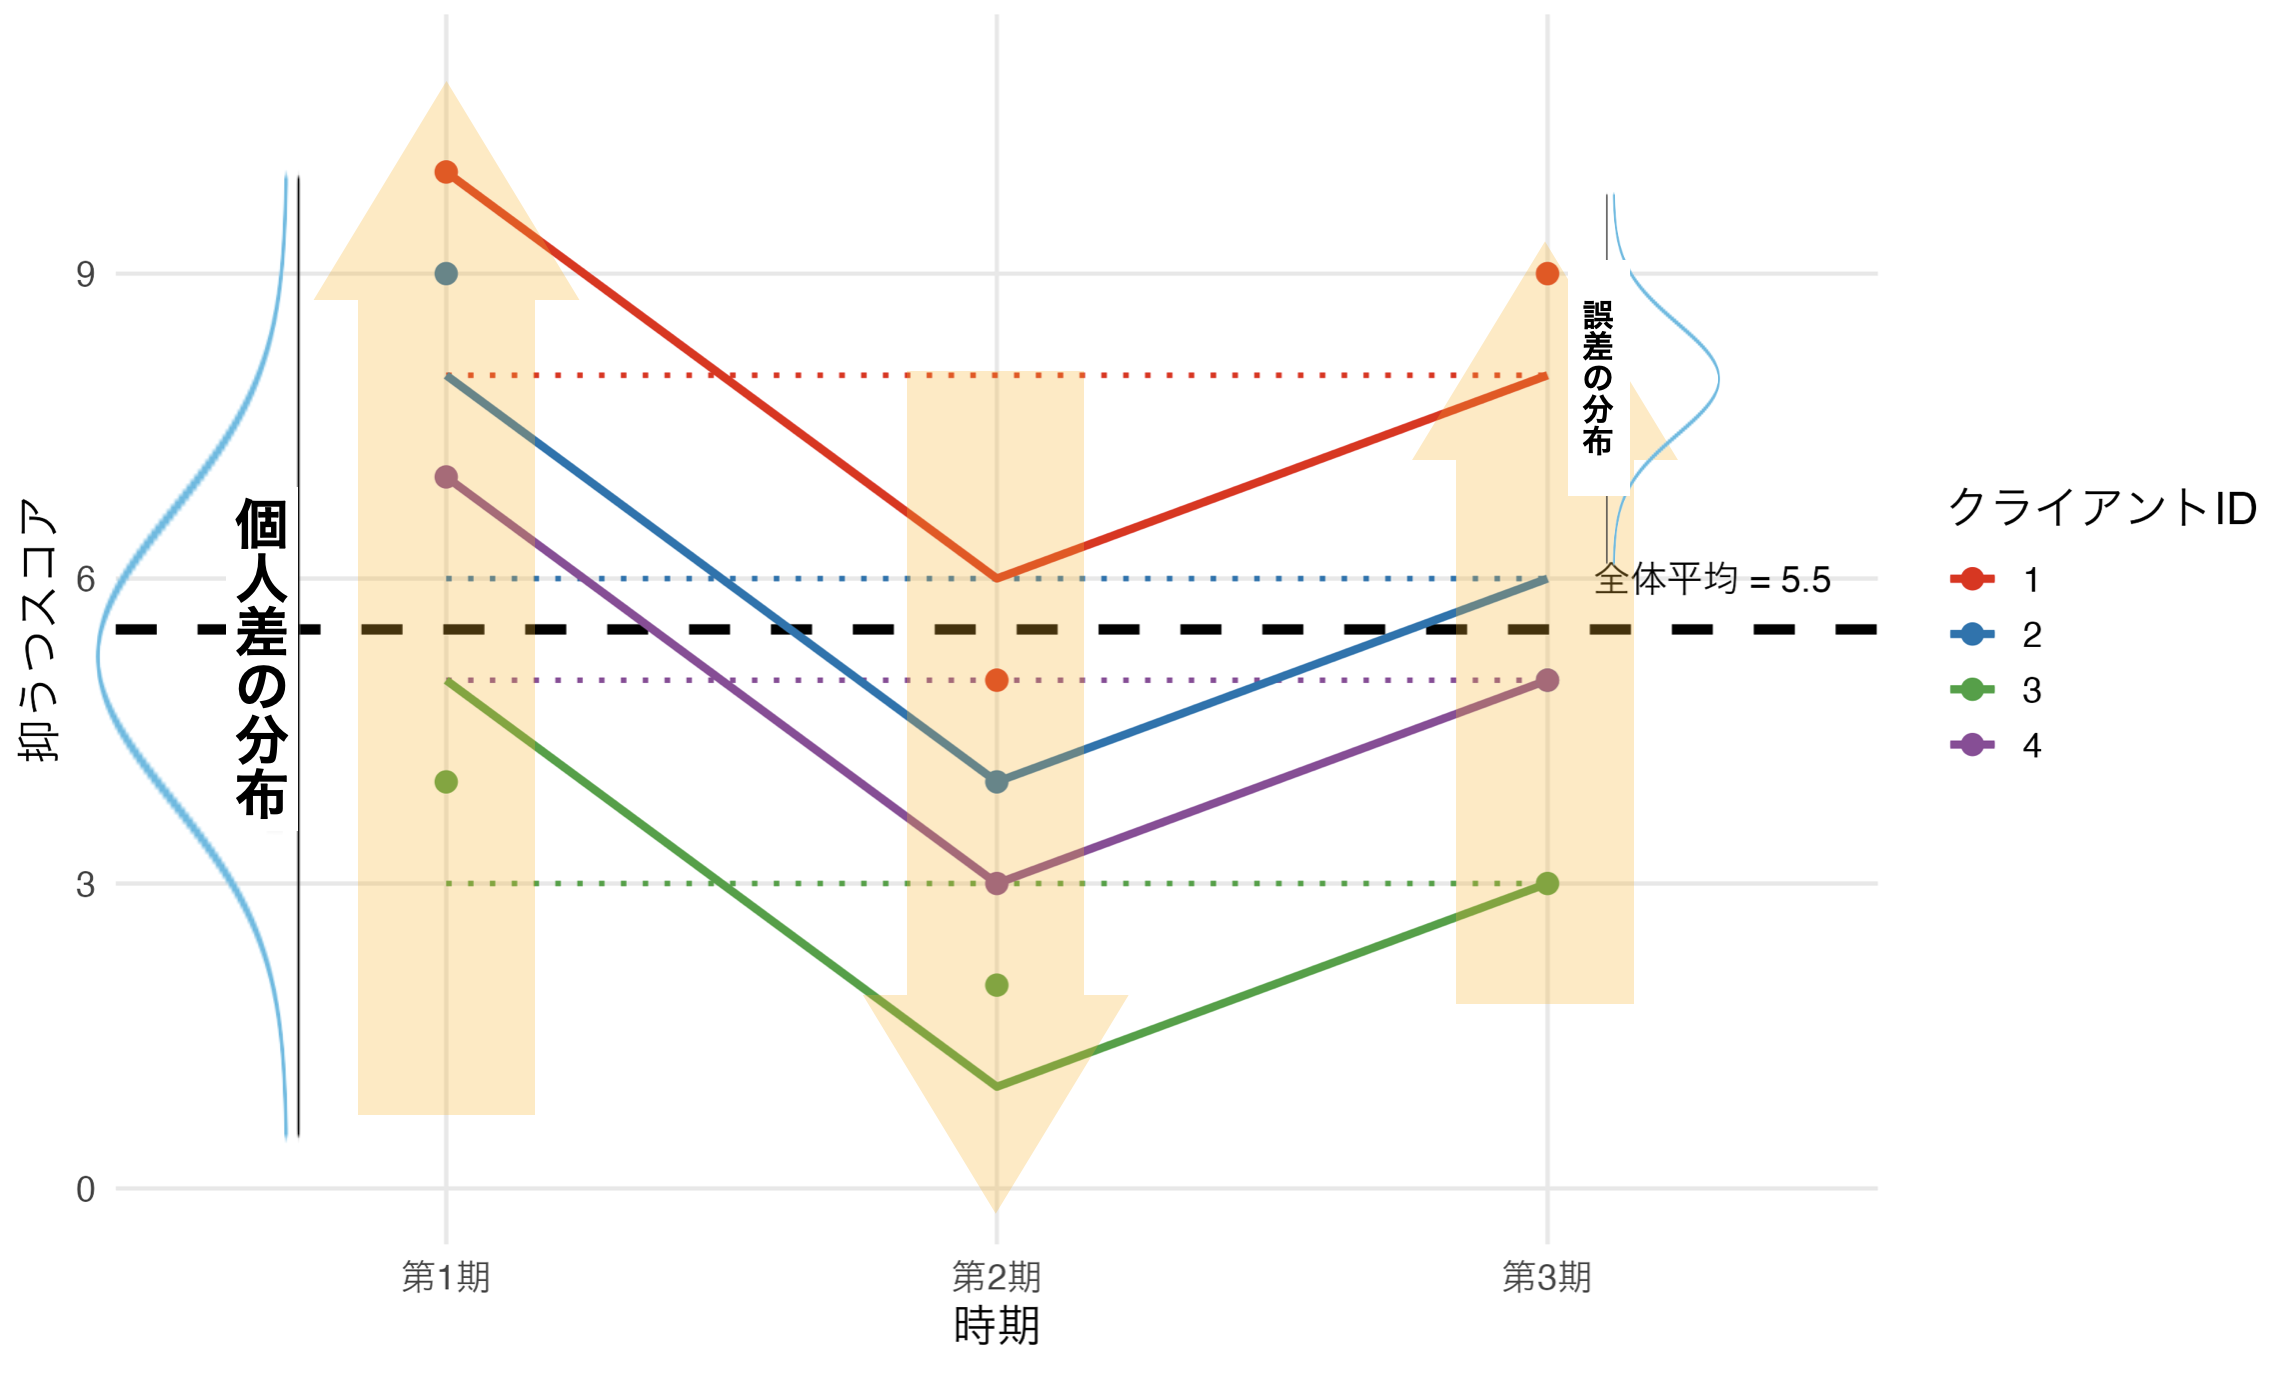
\includegraphics[keepaspectratio,width=0.85\linewidth]{figures/21_Within/mixed_model.png}
    \caption{混合効果モデルのイメージ}
    \label{fig:21_06}
\end{figure}

図で表すとかえってわかりにくくなったかもしれませんが，ポイントは，群内計画では個人差も確率的に変化する要素として捉えられる，ということです。さらに言えば，確率的な要素として考えるということは各個体・各実現値ひとつひとつの個性を考えるのではなく，それらは相互に交換可能な偶然の要素であり，全体的な傾向に従っていると考えることでもあります。

今回は個人差の要素として考えましたが，実験計画では「等価な刺激」を複数用意して，それらをランダムに割り当てる，ということもよく行います。例えば記憶の実験として，無意味綴りの単語を覚えてもらって，幾つ覚えられたかを調べる，ということを考えます。実験参加者は「めぬそ」「きたへ」など，全く意味のない単語を覚えるわけですが，全員が同じものを同じ順番で覚える必要はありません。三文字のひらがなで意味を成さない組み合わせ，という条件を満たす単語を複数用意し，それらをランダムに割り当てることで，刺激の個性を抑え，実験参加者の個性も抑えることができます。このような場合も，刺激の個性は確率的に変化する要素として捉えられるわけです。この刺激グループの各要素が持つ個性も，個人差と同じように正規分布に従うと考えられますから，混合効果モデルとして扱います。

このように個人差も刺激の個性も，さらには実験を行う日や場所なども，確率的に変化する要素として捉えられるわけです。これらすべてを混合効果モデルとして扱うことも可能であり，実際にそういう分析手法も存在します(線形混合モデル，Linear Mixed Modelなど)。例えば同じ実験を複数の国や地域，実験室で行ったものを統合した\keyterm{メタ分析}{めたぶんせき}{meta analysis}などでは，実験室ごとの違いも確率的に変化する要素として捉え，混合効果モデルで分析することがあります。ここでは詳細には立ち入りませんが，実験計画法の理論がこのように発展していることを知っておいてください。

もっともっと面白いことを言えば，係数$\beta$も確率的に変化する要素として捉えることもできます。いろいろな効果の現れ方が，個人や集団，実験室ごと，あるいは地域や国ごとに少しずつ異なるということも考えられるでしょう。もちろん全体的な効果はありますが，それに加えてローカルな影響があり，それが切片だけでなく傾きにも現れているかもしれません。このように考えるモデルは\keyterm{階層線形モデル}{かいそうせんけいもでる}{hierarchical linear model}などと呼ばれ，ベイズ統計学の枠組みで扱われることが多いです。ここでは詳細には立ち入りませんが，実験計画法の理論がこのように発展していることを知っておいてください。

\section{課題}
\paragraph{Within計画の分析例}本講で扱ったのと同じような，一要因3水準Within計画のデータを表\ref{m14_example}のように用意しました。要因の効果，個人差，誤差の大きさ(平方和)を計算する練習をしてみましょう。
\begin{table}[h]
	\centering
	\caption{効果，個人差，誤差の計算練習}
	\begin{tabular}{l|ccc}
		\hline
		ID & Time1 & Time2 & Time3 \\
		\hline
		A  & 48    & 48    & 40    \\
		B  & 49    & 51    & 45    \\
		C  & 58    & 59    & 46    \\
		D  & 46    & 44    & 37    \\
		E  & 52    & 52    & 46    \\
		\hline
	\end{tabular}
	\label{m14_example}
\end{table}

\end{document}
